
\hypertarget{cv:registrarAtributo}{\section{Registrar Atributo}} \label{sec:registrarAtributo}

	Esta funcionalidad le permitirá registrar un atributo que perteneciente a una entidad dentro del proyecto que se esta operando. 

		\subsection{Procedimiento}

			%Pasos de procedimiento
			\begin{enumerate}
	
			\item Oprima el botón \IURegistrar{} de la pantalla \ref{fig:GestionarAtributos} ''Gestionar Atributos''.
			
			\item Se mostrará la pantalla \ref{fig:registrarAtributo} ''Registrar Atributo''.

			%Pantalla
			\begin{figure}[H]
				\begin{center}
					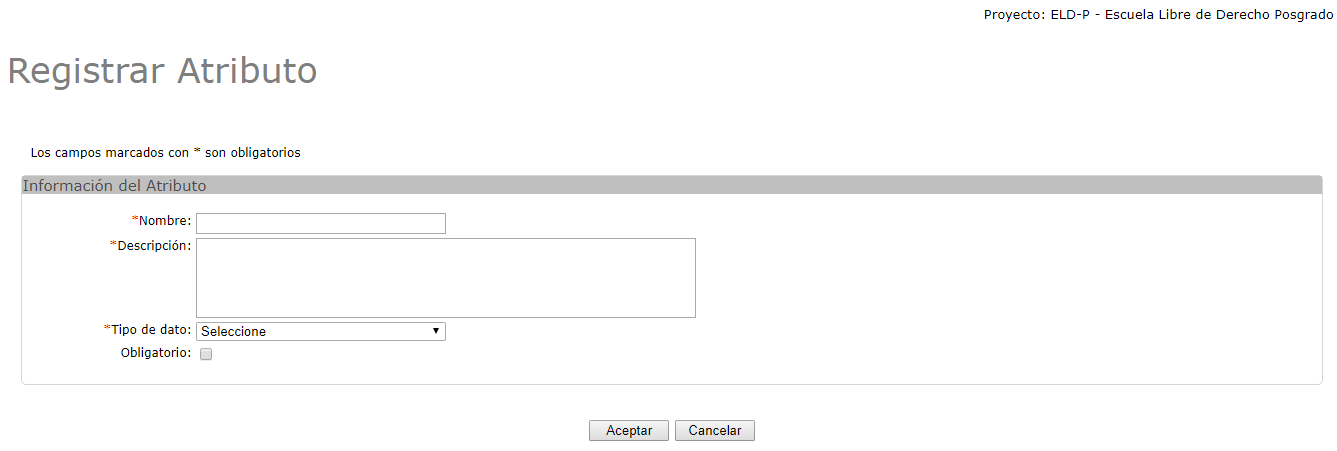
\includegraphics[scale=0.5]{roles/lider/entidades/atributos/pantallas/IU12-1-1registrarAtributo}
					\caption{Registrar Atributo}
					\label{fig:registrarAtributo}
				\end{center}
			\end{figure}
		
			\item Ingrese el nombre, una pequeña descripción, el tipo de dato que aceptará el atributo y marqué si es obligatorio o no.
			
			\item Dependiendo del tipo de dato que elija aparecerán nuevos campos que son requeridos para el tipo de dato seleccionado. Las siguientes pantallas muestran los campos que requiere cada tipo de dato:
			
			\begin{figure}[H]
				\begin{center}
					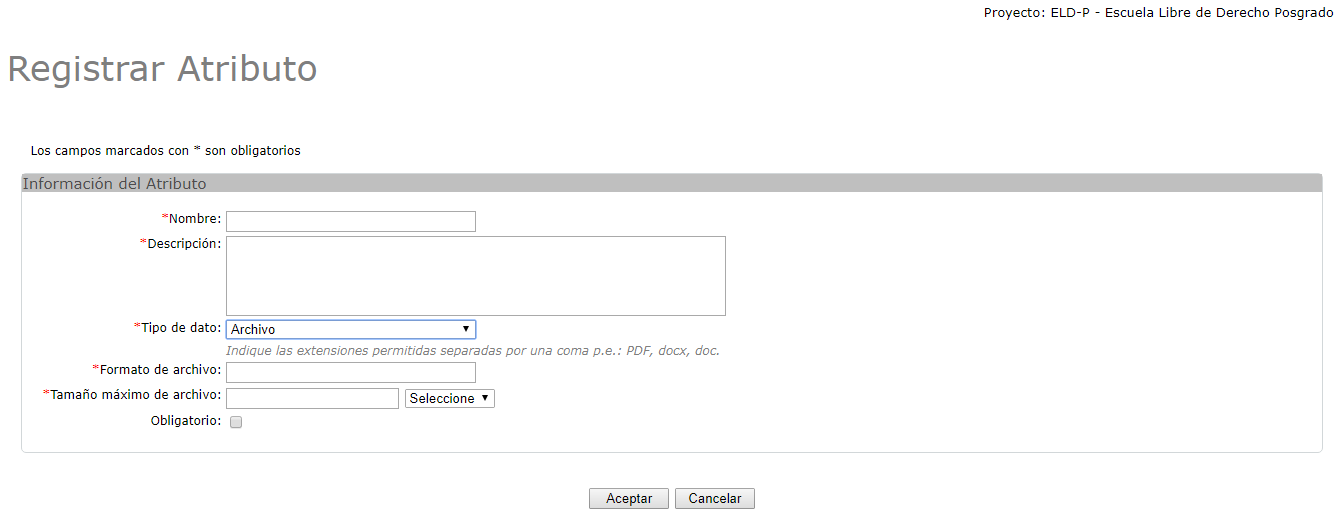
\includegraphics[scale=0.5]{roles/lider/entidades/atributos/pantallas/IU12-1-1AregistrarAtributo}
					\caption{Registrar Atributo: Archivo}
					\label{fig:registrarAtributoA}
				\end{center}
			\end{figure}
		
			\begin{figure}[H]
				\begin{center}
					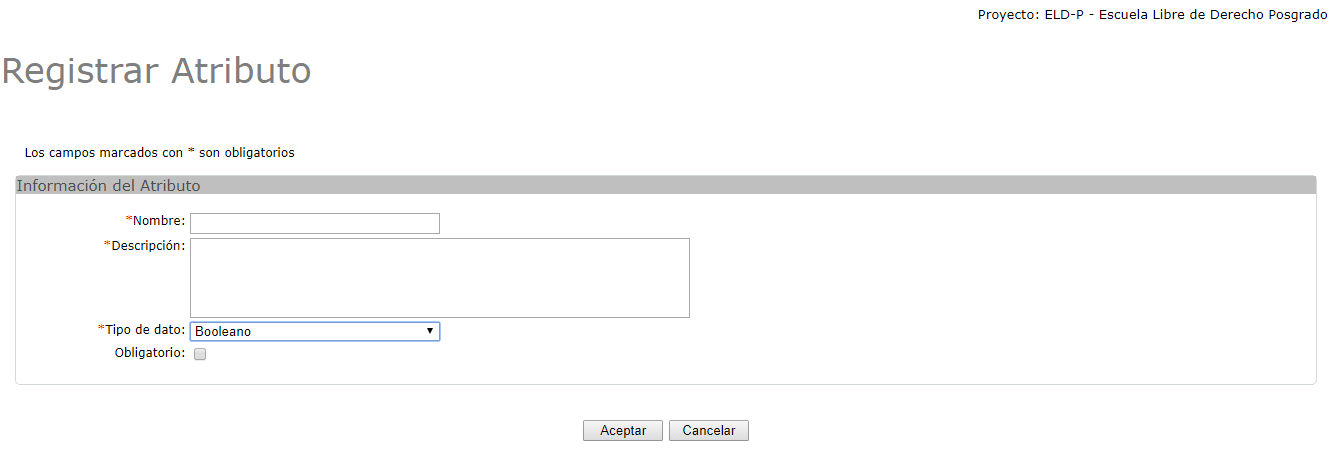
\includegraphics[scale=0.5]{roles/lider/entidades/atributos/pantallas/IU12-1-1BregistrarAtributo}
					\caption{Registrar Atributo: Booleano}
					\label{fig:registrarAtributoB}
				\end{center}
			\end{figure}
		
			\begin{figure}[H]
				\begin{center}
					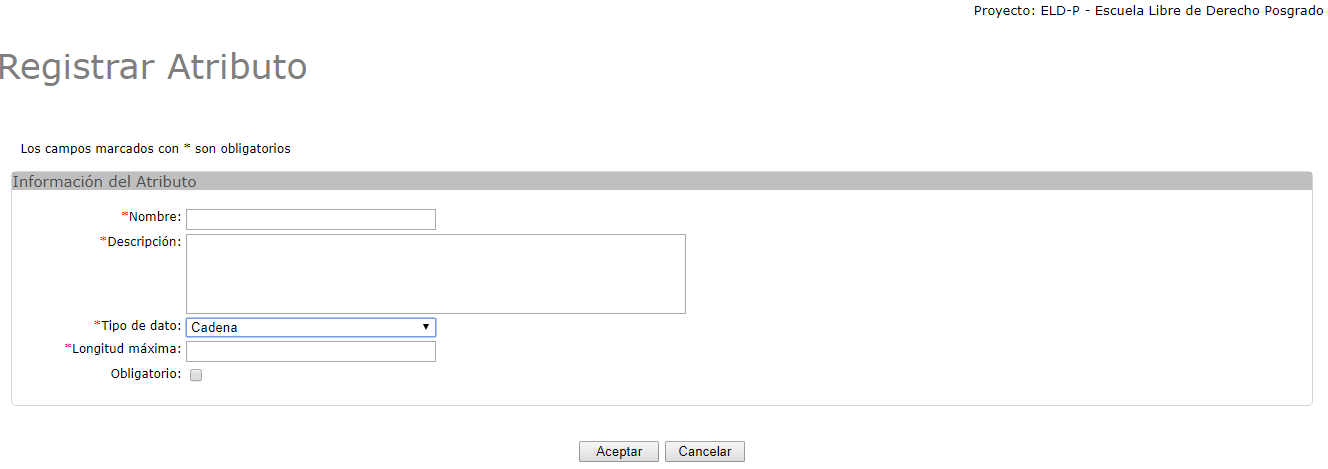
\includegraphics[scale=0.5]{roles/lider/entidades/atributos/pantallas/IU12-1-1CregistrarAtributo}
					\caption{Registrar Atributo: Cadena}
					\label{fig:registrarAtributoC}
				\end{center}
			\end{figure}
		
			\begin{figure}[H]
				\begin{center}
					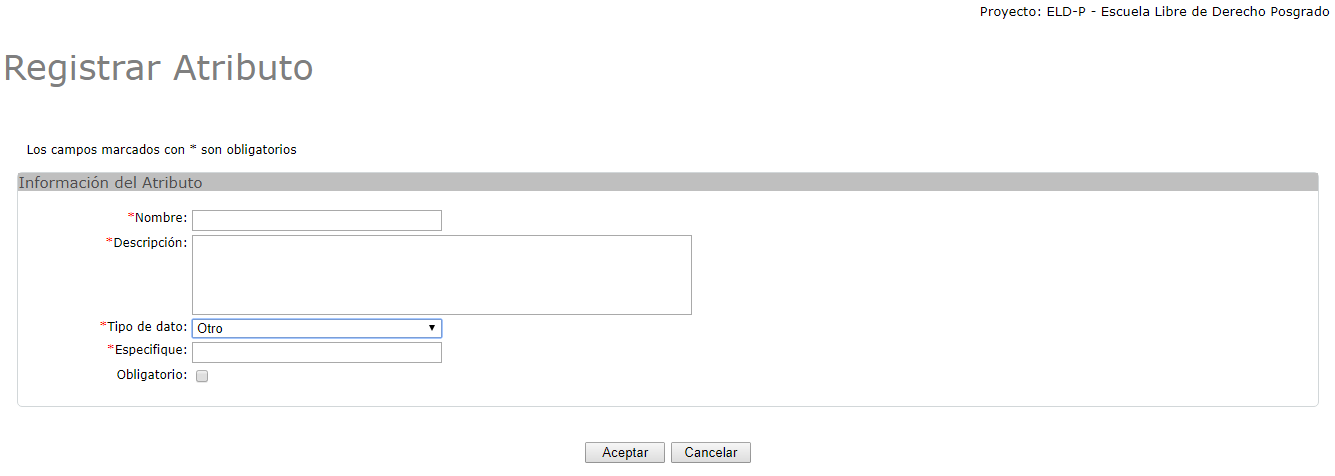
\includegraphics[scale=0.5]{roles/lider/entidades/atributos/pantallas/IU12-1-1DregistrarAtributo}
					\caption{Registrar Atributo: Otro}
					\label{fig:registrarAtributoD}
				\end{center}
			\end{figure}
			
			\item Oprima el botón \IUAceptar.
			
			\item Se mostrará el mensaje \ref{fig:atributoRegistrado} en la pantalla \ref{fig:GestionarAtributos} ''Gestionar Atributos''.
			
			\begin{figure}[htbp!]
				\begin{center}
					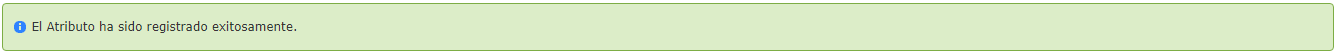
\includegraphics[scale=0.5]{roles/lider/entidades/atributos/pantallas/IU12-1-1MSG1}
					\caption{MSG: Entidad Registrada}
					\label{fig:atributoRegistrado}
				\end{center}
			\end{figure}
			\end{enumerate}